% Volume III: Probability, Statistics, Information, and Causality
% Continuity note for Chapter 13.
% Previous dependencies: Chapter 1's typed objects, statements, quantifiers, and proof habits; Chapter 2's functions, domains, codomains, images, and preimages; Chapters 3-5's vector, matrix, inner-product, and projection geometry; Chapter 11's measurable spaces, measures, densities, null sets, and integration; Chapter 12's function-space viewpoint for signals and operators.
% New durable concepts: probability spaces; sample spaces; events; sigma-algebras as event systems; probability axioms; complements, unions, and inclusion-exclusion; random variables as measurable functions; preimage events; pushforward distributions; CDFs, PMFs, and densities; joint, marginal, and conditional distributions; independence; random vectors; mean vectors; covariance matrices; correlation; positive semidefinite covariance geometry.
% Forward hooks: Chapter 14 reuses distributions as named probability laws; Chapter 15 develops expectation, conditioning, Bayes' theorem, and decisions; Chapter 16 studies convergence and concentration of random quantities; Chapter 17 turns likelihoods and uncertainty into inference; Chapter 18 measures uncertainty and distinguishability with entropy, KL divergence, mutual information, and Fisher geometry.
% Notation commitments: Probability spaces are written (\Omega,\mathcal{F},P); outcomes are \omega; events are A,B,E; random variables are X,Y and their values are x,y; distributions are P_X or p_X; CDFs are F_X; joint mass or density functions are p_{X,Y}; conditional laws are p_{X\mid Y}; random vectors are X\in\mathbb{R}^d with mean \mu=\mathbb{E}[X] and covariance \Sigma=\mathbb{E}[(X-\mu)(X-\mu)^\top].
% Figure plan: four ImageGen raster figures under imagegen-figures/ch13-* are referenced: probability spaces and probability measures for 13.1; random variables as functions and induced distributions for 13.2; joint, marginal, and conditional distributions for 13.3; random vectors and covariance geometry for 13.4.
\section{Chapter 13: Probability Spaces and Random Variables}
\label{ch:probability-spaces-random-variables}

The first two volumes built a language for objects, maps, geometry, approximation, local change, integration, and functions. Chapter 11 already introduced the measure-theoretic machinery needed to assign size to sets. Chapter 12 treated whole signals as mathematical objects. We now put those tools to work on uncertainty.

Probability begins with a simple discipline: say what the possible outcomes are, say which questions about those outcomes count as events, and assign numbers to those events in a consistent way. Random variables then turn raw outcomes into typed quantities we can compute with, such as spike counts, labels, reaction times, losses, or neural population vectors.

\paragraph{Chapter problem.}
How can uncertainty be represented as a probability measure, how do random variables turn outcomes into mathematical data, and how do joint distributions and covariance describe relationships among random quantities?

\paragraph{Section map.}
Section 13.1 defines probability spaces and probability axioms. Section 13.2 treats random variables as measurable functions and explains how they induce distributions. Section 13.3 builds joint, marginal, conditional, and independent distributions. Section 13.4 extends the language to random vectors, mean vectors, covariance matrices, and covariance geometry.

\subsection{13.1 Probability as measure of uncertainty}

\paragraph{Motivating question.}
What mathematical object assigns probabilities to uncertain events while preserving the rules for complements, unions, and disjoint alternatives?

\paragraph{Beginner setup.}
Probability is a measure of uncertainty. It assigns numbers between \(0\) and \(1\) to events. An event is not a vague sentence floating by itself; it is a subset of a specified outcome space. If the experiment is two fair coin tosses, the sample space is
\[
\Omega=\{HH,HT,TH,TT\}.
\]
The event "at least one head" is the subset
\[
A=\{HH,HT,TH\}.
\]
For fair coins, \(P(A)=3/4\). The event "no heads" is the complement \(A^c=\{TT\}\), with probability \(1/4\).

The smallest nontrivial example already shows the main structure. We choose possible outcomes, choose events, and assign probabilities. On a finite fair sample space, the probability of an event is the number of favorable outcomes divided by the total number of outcomes. In more general models, probabilities may come from a density, a fitted model, a subjective prior, or empirical frequencies. The mathematical rules are the same.

Probability solves a modeling problem: before the outcome is observed, many outcomes are possible. A probability measure describes how uncertainty is distributed across events. In a neural experiment, the uncertain outcome may be a spike train. In supervised learning, it may be a data-label pair. In a latent-variable model, it may include both observed data and hidden causes.

What to keep in mind: probabilities attach to events in a specified model. A probability is not automatically a long-run frequency, not automatically a personal belief, and not automatically a physical property of the world. Those are interpretations. The mathematical object is a probability measure \(P\) on a space of events.

\begin{figure}[htbp]
\centering
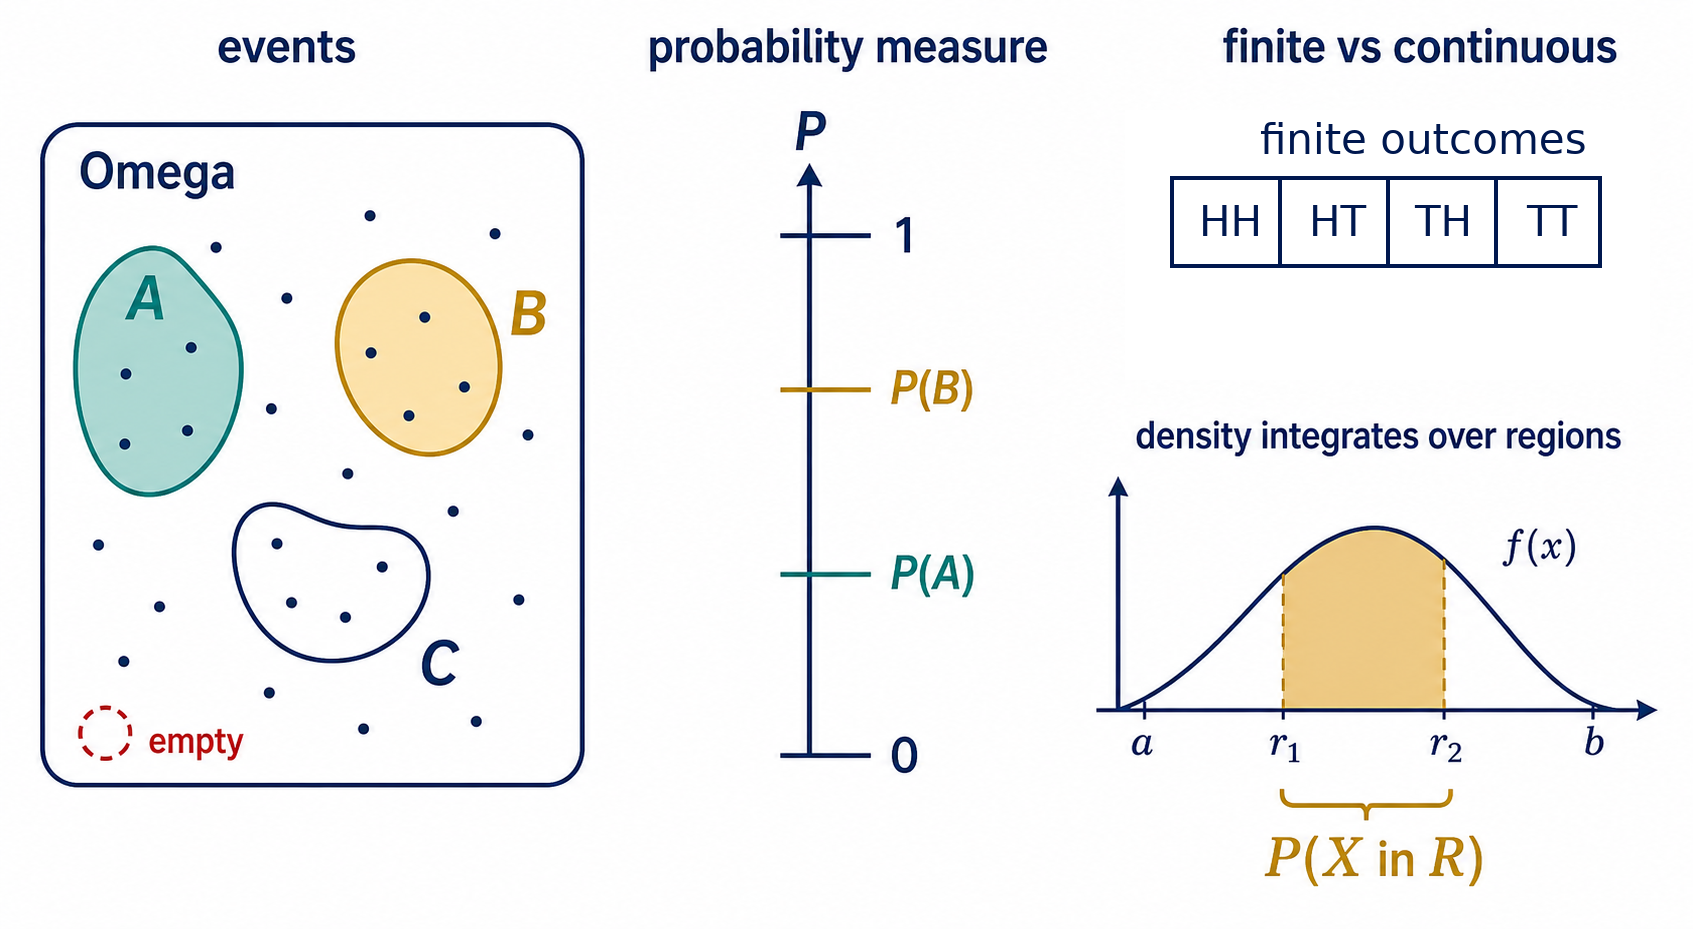
\includegraphics[width=0.98\linewidth]{imagegen-figures/ch13-probability-space.png}
\caption{A probability model has outcomes \(\Omega\), events such as \(A\), \(B\), and \(C\), and a probability measure \(P\) assigning numbers to events. Finite models often assign mass to individual outcomes. Continuous models usually assign probability to regions by integrating a density over the region.}
\label{fig:ch13-probability-space}
\end{figure}

\paragraph{Formal setup.}
A probability space is a triple
\[
(\Omega,\mathcal{F},P).
\]
Here \(\Omega\) is the sample space, whose elements \(\omega\in\Omega\) are outcomes. The collection \(\mathcal{F}\) is a \(\sigma\)-algebra of subsets of \(\Omega\); its elements are the events whose probabilities are defined. The function
\[
P:\mathcal{F}\to[0,1]
\]
is a probability measure satisfying
\[
P(\Omega)=1,
\qquad
P(\emptyset)=0,
\]
and countable additivity: if \(A_1,A_2,\ldots\in\mathcal{F}\) are pairwise disjoint, then
\[
P\!\left(\bigcup_{i=1}^{\infty}A_i\right)
=
\sum_{i=1}^{\infty}P(A_i).
\]
The central finite rule for this section is inclusion-exclusion:
\[
\boxed{P(A\cup B)=P(A)+P(B)-P(A\cap B).}
\]
It corrects the double-counting that occurs when two events overlap.

When \(\Omega\) is finite and all subsets are allowed events, \(\mathcal{F}=2^\Omega\). When \(\Omega=\mathbb{R}\) or \(\mathbb{R}^d\), \(\mathcal{F}\) is usually a Borel \(\sigma\)-algebra or a completion of it. In continuous models, probabilities of regions often have the form
\[
P(E)=\int_E p(\omega)\,d\omega,
\]
where \(p\) is a density. This integral notation is a special representation of a probability measure, not the definition of probability itself.

\paragraph{Core intuition.}
Figure~\ref{fig:ch13-probability-space} separates three layers. The rectangle of outcomes represents \(\Omega\). The colored regions are events. The vertical scale represents \(P\), the rule that assigns numerical uncertainty to those events. The drawing area of an event is not necessarily its probability; the probability is whatever the model assigns.

The axioms are bookkeeping rules for uncertainty. If an event and its complement cover all possibilities without overlap, their probabilities must add to \(1\). If two events are disjoint alternatives, the probability that either occurs should be the sum of their probabilities. If events overlap, inclusion-exclusion subtracts the overlap once because \(P(A)+P(B)\) counts \(A\cap B\) twice.

Common misconceptions are worth clearing early. First, probability zero does not always mean impossible. In a continuous distribution on \([0,1]\), the event \(\{0.37\}\) has probability zero, but \(0.37\) is still a legitimate value. Second, outcomes do not have to be equally likely. A sample space lists possibilities; the probability measure assigns weights. Third, probability is not the same thing as a density. A density must be integrated over a region before it becomes a probability.

This section reuses Chapter 11's measure language. It prepares Section 13.2, where questions such as \(\{X\leq t\}\) become events through preimages, and it prepares later chapters where probabilities become likelihoods, priors, posterior distributions, and information measures.

\paragraph{Main theorem: complements and inclusion-exclusion.}
For events \(A,B\in\mathcal{F}\),
\[
P(A^c)=1-P(A)
\]
and
\[
P(A\cup B)=P(A)+P(B)-P(A\cap B).
\]

\emph{Proof sketch.}
The sample space decomposes into the disjoint union
\[
\Omega=A\cup A^c.
\]
By additivity,
\[
1=P(\Omega)=P(A)+P(A^c),
\]
so \(P(A^c)=1-P(A)\).

For inclusion-exclusion, decompose \(A\cup B\) into three disjoint pieces:
\[
A\cup B
=
(A\setminus B)\cup(A\cap B)\cup(B\setminus A).
\]
Additivity gives
\[
P(A\cup B)
=P(A\setminus B)+P(A\cap B)+P(B\setminus A).
\]
Also,
\[
P(A)=P(A\setminus B)+P(A\cap B),
\qquad
P(B)=P(B\setminus A)+P(A\cap B).
\]
Adding \(P(A)+P(B)\) counts the overlap \(A\cap B\) twice, so subtracting \(P(A\cap B)\) leaves exactly \(P(A\cup B)\). The mechanism is the same as finite area bookkeeping, but it follows from the measure axioms.

\paragraph{Worked examples.}
\emph{Small finite example.} Roll a fair six-sided die. Let
\[
A=\{2,4,6\}
\]
be the event "even" and
\[
B=\{5,6\}
\]
be the event "greater than four." Then \(P(A)=3/6\), \(P(B)=2/6\), and \(A\cap B=\{6\}\), so
\[
P(A\cup B)=\frac{3}{6}+\frac{2}{6}-\frac{1}{6}=\frac{4}{6}.
\]
The event \(A\cup B=\{2,4,5,6\}\) indeed has four outcomes.

\emph{ML/neuroscience example.} In a spike-count experiment, let \(\Omega\) be all possible trial records during a \(100\) ms window: stimulus identity, spike times, and measurement noise. The event
\[
A=\{\text{at least five spikes occur in the window}\}
\]
is a subset of \(\Omega\). A model \(P\) might assign \(P(A)=0.18\) under a weak stimulus and \(P(A)=0.71\) under a strong stimulus. The mathematical objects are explicit: outcomes are full trial records, the event is a set of records satisfying a spike-count condition, and the probability measure describes uncertainty about which record will occur.

\paragraph{ML/DL/neuroscience connections.}
In supervised learning, \(\Omega\) can be the set of possible pairs \((x,y)\), where \(x\) is an input and \(y\) is a label. Events include \(y=1\), \(x\) lying in a region of feature space, or a trained classifier making an error. The probability measure may be the true data-generating distribution, an empirical distribution over a dataset, or a parametric model. In neuroscience, \(\Omega\) can be a space of stimuli and neural responses; events become spike-count ranges, reaction-time intervals, or regions of population activity. Probability as measure lets all of these cases use the same notation.

\paragraph{Exercises.}
\begin{enumerate}[label=\textbf{13.1.\arabic*.}, leftmargin=*]
\item \textbf{Mechanical.} A fair die is rolled. Let \(A=\{1,2,3\}\) and \(B=\{3,4\}\). Compute \(P(A)\), \(P(B)\), \(P(A\cap B)\), \(P(A\cup B)\), and \(P(A^c)\).
\item \textbf{Proof or derivation.} Prove that if \(A\subseteq B\), then \(P(A)\leq P(B)\). Hint: write \(B\) as a disjoint union involving \(A\).
\item \textbf{Numerical/computational.} In \(500\) trials, a neuron fires at least five spikes in \(91\) trials. Treat empirical frequency as a probability measure on the finite set of trials. Estimate the probability of the event "at least five spikes."
\item \textbf{Interpretation.} In a continuous model for a reaction time \(T\), why can \(P(T=0.327)=0\) while reaction times near \(0.327\) seconds remain likely?
\item \textbf{Debug the misconception.} A student says, "The sample space lists four outcomes, so each outcome must have probability \(1/4\)." Explain why the sample space alone does not determine the probability measure.
\end{enumerate}

\subsection{13.2 Random variables as measurable functions}

\paragraph{Motivating question.}
If outcomes can be coin toss sequences, trial records, or neural recordings, how do we turn them into numerical quantities such as counts, labels, losses, or response amplitudes?

\paragraph{Beginner setup.}
A random variable is a function on the sample space. It takes an outcome \(\omega\) and returns a value. The randomness comes from not knowing which outcome will occur; the function itself is fixed once the model is specified.

For two coin tosses, let
\[
\Omega=\{HH,HT,TH,TT\}
\]
and define \(X(\omega)\) to be the number of heads:
\[
X(HH)=2,\qquad
X(HT)=1,\qquad
X(TH)=1,\qquad
X(TT)=0.
\]
The event \(\{X=1\}\) is not a new primitive object. It is the preimage
\[
X^{-1}(\{1\})=\{HT,TH\}.
\]
If the coins are fair, then \(P(X=1)=P(\{HT,TH\})=1/2\).

Random variables solve the problem of extracting typed data from raw outcomes. A trial outcome may contain a full voltage trace, a stimulus, eye position, and many spike times. A random variable might keep only the spike count in one time bin, the stimulus category, the reaction time, or the model loss on that trial.

What to keep in mind: a random variable is not necessarily a scalar and not necessarily continuous. It can be discrete, continuous, vector-valued, category-valued, or function-valued. The key requirement is measurability: events about its values must correspond to legitimate events in the original sample space.

\begin{figure}[htbp]
\centering
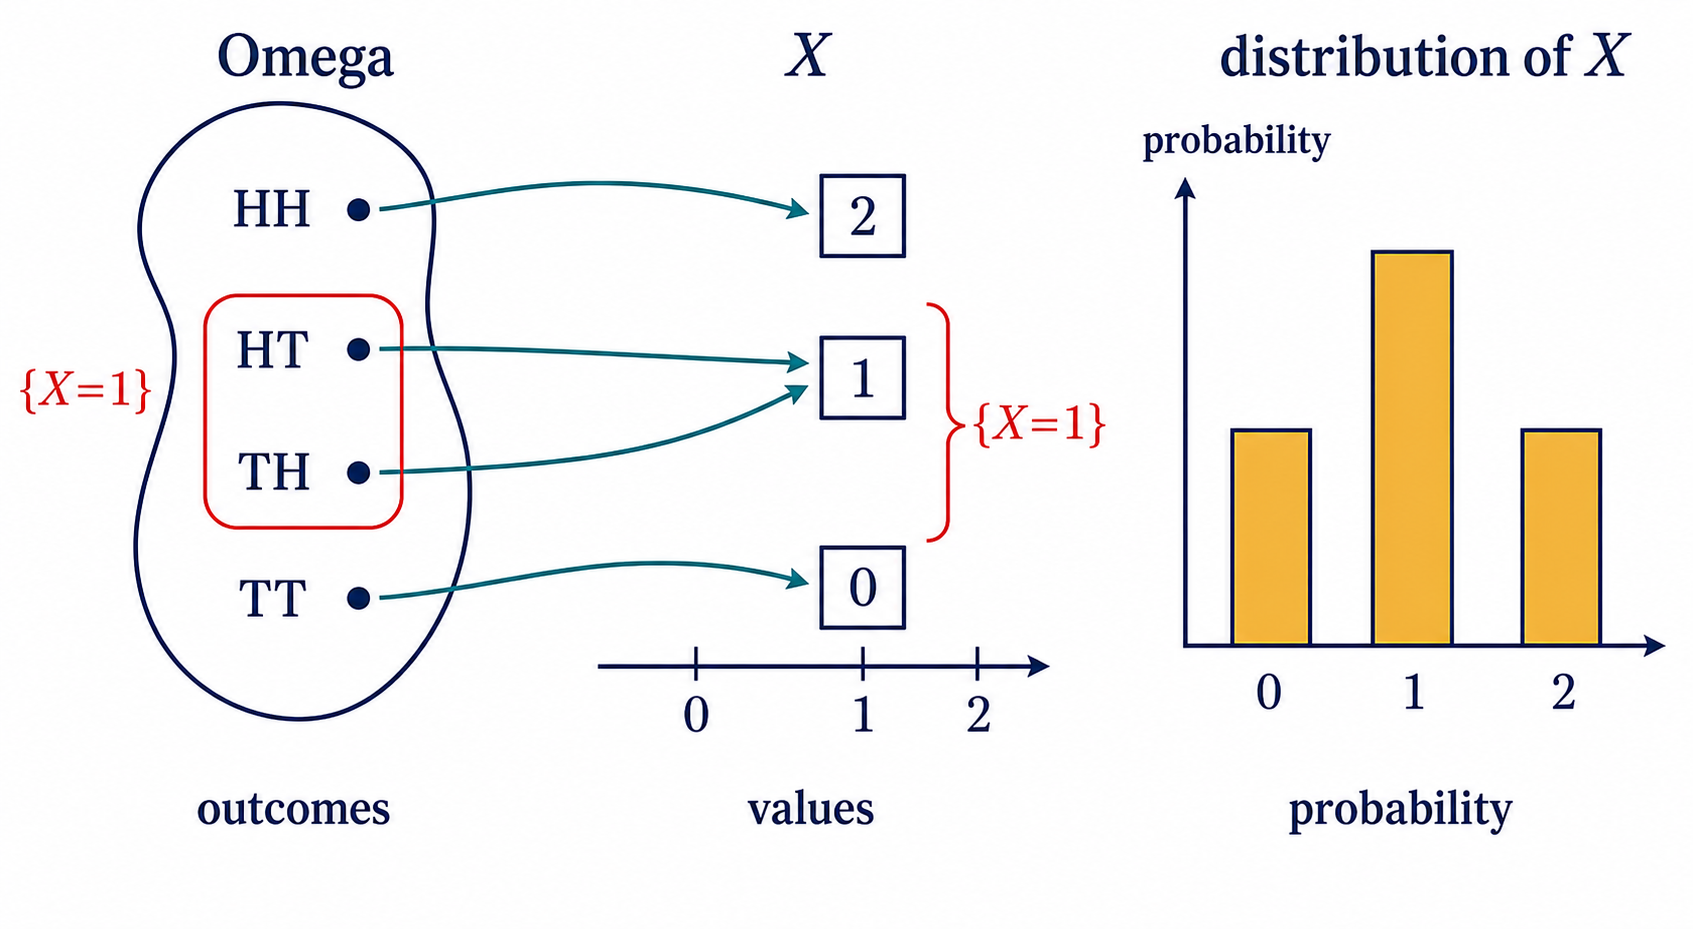
\includegraphics[width=0.98\linewidth]{imagegen-figures/ch13-random-variable-function-v2.png}
\caption{A random variable \(X\) is a function from outcomes to values. For two coin tosses, \(X\) can count the number of heads. The event \(\{X=1\}\) is the preimage \(\{HT,TH\}\) in the sample space. The distribution of \(X\) records the probabilities of the values \(0\), \(1\), and \(2\).}
\label{fig:ch13-random-variable-function}
\end{figure}

\paragraph{Formal setup.}
Let \((\Omega,\mathcal{F},P)\) be a probability space and let \((S,\mathcal{S})\) be a measurable value space. A random variable is a measurable function
\[
X:(\Omega,\mathcal{F})\to(S,\mathcal{S}).
\]
Measurability means that for every measurable set \(B\in\mathcal{S}\),
\[
X^{-1}(B)=\{\omega\in\Omega:X(\omega)\in B\}\in\mathcal{F}.
\]
For a real-valued random variable \(X:\Omega\to\mathbb{R}\), it is enough in many standard settings to check that events of the form
\[
\{X\leq t\}
\]
are measurable for every real \(t\).

The distribution of \(X\), also called the law of \(X\), is the probability measure \(P_X\) on \(S\) defined by the pushforward equation
\[
\boxed{P_X(B)=P(X\in B)=P\!\left(X^{-1}(B)\right).}
\]
For a real-valued \(X\), the cumulative distribution function is
\[
F_X(t)=P(X\leq t).
\]
If \(X\) is discrete, its probability mass function is
\[
p_X(x)=P(X=x).
\]
If \(X\) is continuous with density \(p_X\), then
\[
P(X\in B)=\int_B p_X(x)\,dx.
\]

\paragraph{Core intuition.}
Figure~\ref{fig:ch13-random-variable-function} shows the central idea from Chapter 2 returning in probability form: functions create preimages. An event in value space, such as \(\{1\}\), pulls back to an event in outcome space, such as \(\{HT,TH\}\). The probability of the value event is the probability of that preimage.

This viewpoint prevents several beginner errors. A random variable is not a container holding a randomly changing number. It is a map from outcomes to values. A realized value, such as \(X=1\), is what we see after an outcome occurs. The distribution \(P_X\) is not the same thing as the function \(X\); many different random variables on different sample spaces can have the same distribution.

Measurability is the technical condition that makes questions about \(X\) legal. If \(B\) is a value-space event, \(X^{-1}(B)\) must be an event in \(\mathcal{F}\), otherwise \(P(X\in B)\) would not be defined. In everyday finite examples this condition is automatic. In continuous and function-valued models it is the reason probability works cleanly with limits, integrals, and transformations.

This section connects backward to Chapter 2's domain/codomain discipline and Chapter 11's measurable functions. It connects forward to Chapter 14, where \(P_X\) will be named by familiar distributions, and to Chapter 15, where expectations and conditional expectations are operators applied to random variables.

\paragraph{Main theorem: pushforward distributions are probability measures.}
Let \(X:(\Omega,\mathcal{F},P)\to(S,\mathcal{S})\) be a random variable. Define
\[
P_X(B)=P(X^{-1}(B))
\]
for \(B\in\mathcal{S}\). Then \(P_X\) is a probability measure on \((S,\mathcal{S})\).

\emph{Proof sketch.}
First, \(P_X(B)\geq0\) because \(P\) is nonnegative. Second,
\[
P_X(S)=P(X^{-1}(S))=P(\Omega)=1,
\]
because every outcome maps into the value space \(S\). Third, suppose \(B_1,B_2,\ldots\in\mathcal{S}\) are pairwise disjoint. Preimages preserve unions and disjointness:
\[
X^{-1}\!\left(\bigcup_{i=1}^{\infty}B_i\right)
=
\bigcup_{i=1}^{\infty}X^{-1}(B_i),
\]
and the sets \(X^{-1}(B_i)\) are pairwise disjoint. Countable additivity of \(P\) gives
\[
P_X\!\left(\bigcup_{i=1}^{\infty}B_i\right)
=
P\!\left(\bigcup_{i=1}^{\infty}X^{-1}(B_i)\right)
=
\sum_{i=1}^{\infty}P(X^{-1}(B_i))
=
\sum_{i=1}^{\infty}P_X(B_i).
\]
Thus \(P_X\) obeys the probability axioms. The mechanism is simple: the random variable transports probability from outcomes to values by preimages.

\paragraph{Worked examples.}
\emph{Small finite example.} For two fair coin tosses and \(X=\) number of heads,
\[
p_X(0)=P(X=0)=P(\{TT\})=\frac14,
\]
\[
p_X(1)=P(X=1)=P(\{HT,TH\})=\frac12,
\]
and
\[
p_X(2)=P(X=2)=P(\{HH\})=\frac14.
\]
The CDF is
\[
F_X(t)=
\begin{cases}
0, & t<0,\\
1/4, & 0\leq t<1,\\
3/4, & 1\leq t<2,\\
1, & t\geq2.
\end{cases}
\]

\emph{ML/neuroscience example.} Let \(\Omega\) be full experimental trials. For each trial \(\omega\), define
\[
X(\omega)=\text{number of spikes from neuron 1 in the first }100\text{ ms}.
\]
This random variable maps a rich trial record to a nonnegative integer. The event \(\{X\geq5\}\) is the set of trials with at least five spikes. Its probability can be estimated from data or predicted by a spike-count model. A second random variable \(Y(\omega)\) might be the stimulus identity or the behavioral choice on the same trial.

\paragraph{ML/DL/neuroscience connections.}
In supervised learning, the input \(X\), label \(Y\), loss \(L\), and prediction \(\widehat{Y}\) are all random variables on an underlying space of examples and training randomness. The map \(L(\omega)\) turns a sampled example and model state into a number. In neuroscience, a spike count, a binned population vector, a reaction time, and a stimulus label are random variables extracted from the same trial outcome. The distribution \(P_X\) becomes the empirical or modeled response distribution.

\paragraph{Exercises.}
\begin{enumerate}[label=\textbf{13.2.\arabic*.}, leftmargin=*]
\item \textbf{Mechanical.} Let \(\Omega=\{1,2,3,4,5,6\}\) for a fair die and define \(X(\omega)=1\) if \(\omega\) is even and \(X(\omega)=0\) otherwise. Compute \(X^{-1}(\{1\})\), \(X^{-1}(\{0\})\), \(p_X(1)\), and \(p_X(0)\).
\item \textbf{Proof or derivation.} For a random variable \(X:\Omega\to S\), show that \(X^{-1}(B^c)=\left(X^{-1}(B)\right)^c\). Explain why this matters for events about \(X\).
\item \textbf{Numerical/computational.} A dataset contains spike counts \((0,1,1,2,0,3,1,2)\). Treat the list as samples of a discrete random variable. Estimate \(p_X(0)\), \(p_X(1)\), \(p_X(2)\), and \(p_X(3)\).
\item \textbf{Interpretation.} Two different experiments produce random variables with the same distribution over \(\{0,1,2\}\). What information is captured by the distribution, and what information about the underlying outcomes may be lost?
\item \textbf{Debug the misconception.} A student says, "A random variable is random because the function changes every time." Correct the statement using the outcome \(\omega\) and the function \(X(\omega)\).
\end{enumerate}

\subsection{13.3 Joint, marginal, and conditional distributions}

\paragraph{Motivating question.}
How can we describe two random quantities together, ignore one of them when needed, or update uncertainty about one after observing the other?

\paragraph{Beginner setup.}
Many scientific questions involve relationships between random variables. A stimulus and a neural response occur on the same trial. An image and its label occur in the same example. A latent state and an observation occur in the same model. The joint distribution describes their co-occurrence.

For two discrete random variables \(X\) and \(Y\), a joint table lists probabilities such as
\[
p_{X,Y}(x,y)=P(X=x,Y=y).
\]
The marginal distribution of \(X\) is obtained by summing over all values of \(Y\). The conditional distribution of \(X\) given \(Y=y\) is obtained by restricting attention to the slice where \(Y=y\) and renormalizing.

The smallest nontrivial example is a \(2\times2\) table for two binary variables. If the rows are values of \(X\) and the columns are values of \(Y\), then each cell is one joint probability. Row sums give probabilities for \(X\). Column sums give probabilities for \(Y\). A column normalized by its total gives a conditional distribution of \(X\) given that column's \(Y\)-value.

What to keep in mind: marginalization discards information about the other variable, conditioning uses information about the other variable, and independence says the joint distribution contains no interaction beyond the two marginals.

\begin{figure}[htbp]
\centering
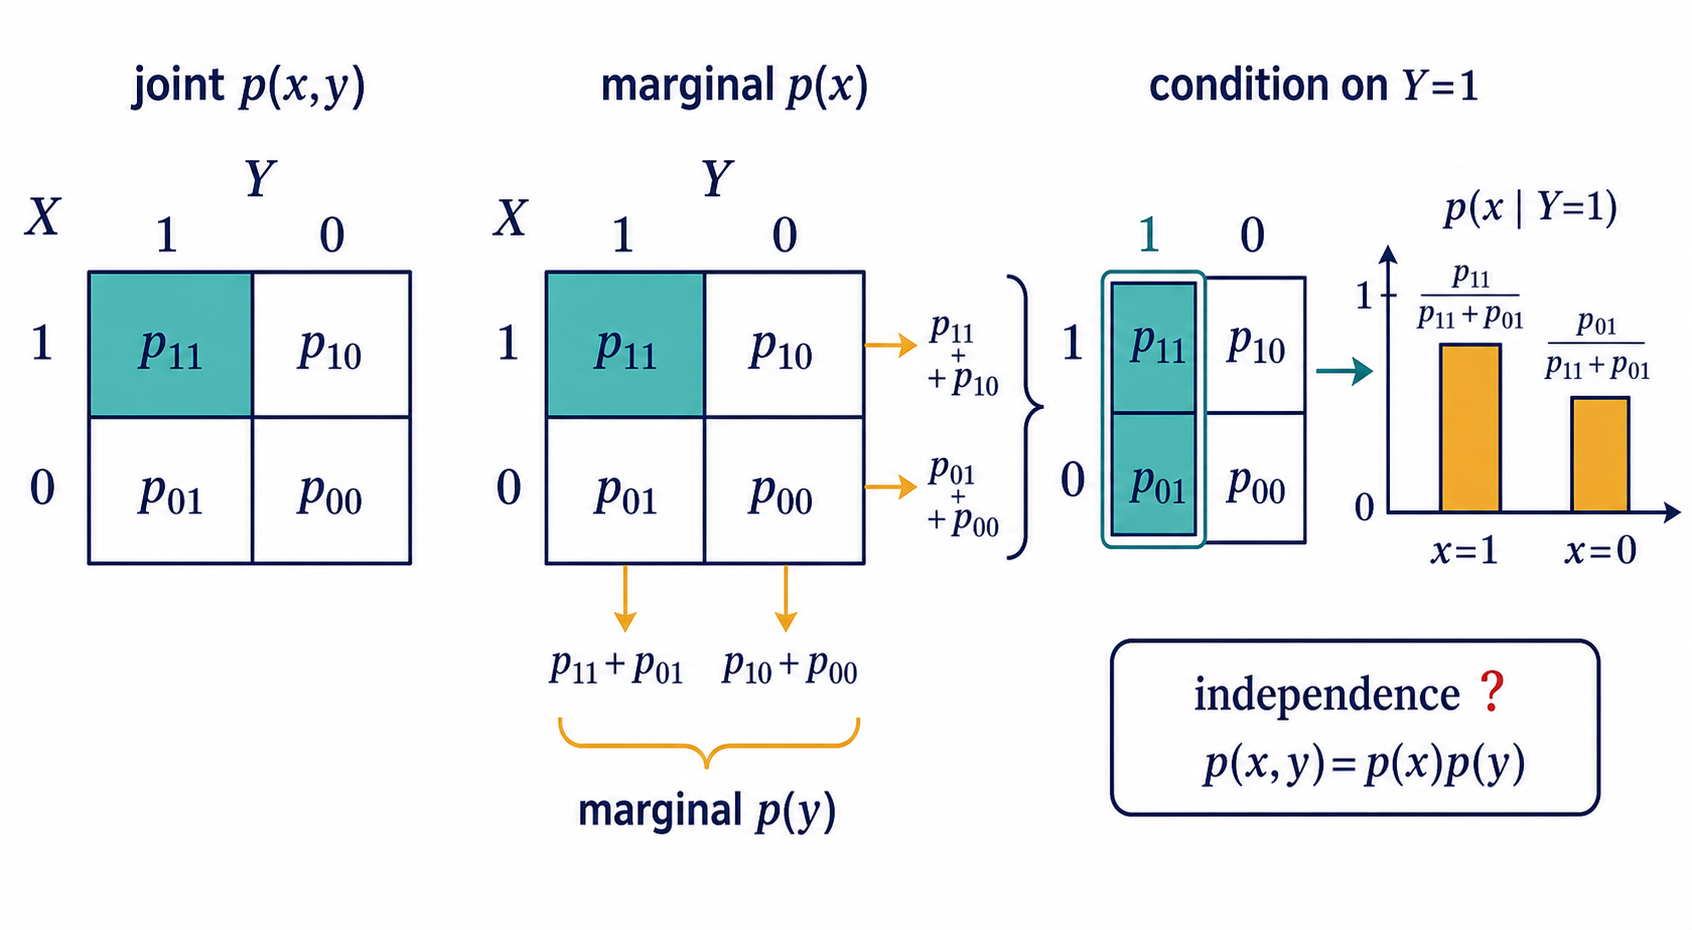
\includegraphics[width=0.98\linewidth]{imagegen-figures/ch13-joint-marginal-conditional.png}
\caption{A joint table stores probabilities for pairs \((X,Y)\). Marginal distributions come from summing rows or columns. A conditional distribution is a selected row or column slice normalized by its total probability. Independence is the special case where joint probabilities factor into marginal probabilities.}
\label{fig:ch13-joint-marginal-conditional}
\end{figure}

\paragraph{Formal setup.}
Let \(X:(\Omega,\mathcal{F})\to(S_X,\mathcal{S}_X)\) and \(Y:(\Omega,\mathcal{F})\to(S_Y,\mathcal{S}_Y)\) be random variables. The pair
\[
(X,Y):\Omega\to S_X\times S_Y,
\qquad
(X,Y)(\omega)=(X(\omega),Y(\omega)),
\]
is itself a random variable into the product value space \((S_X\times S_Y,\mathcal{S}_X\otimes\mathcal{S}_Y)\). Its law is the joint distribution \(P_{X,Y}\), defined for measurable \(C\subseteq S_X\times S_Y\) by
\[
P_{X,Y}(C)=P((X,Y)\in C).
\]
For measurable rectangles \(A\times B\), with \(A\in\mathcal{S}_X\) and \(B\in\mathcal{S}_Y\), this becomes
\[
P_{X,Y}(A\times B)=P(X\in A,\;Y\in B).
\]
For discrete variables, the joint mass function is
\[
p_{X,Y}(x,y)=P(X=x,\;Y=y).
\]
The marginal mass functions are
\[
\boxed{p_X(x)=\sum_y p_{X,Y}(x,y),\qquad
p_Y(y)=\sum_x p_{X,Y}(x,y).}
\]
If \(p_Y(y)>0\), the conditional mass function of \(X\) given \(Y=y\) is
\[
\boxed{p_{X\mid Y}(x\mid y)=\frac{p_{X,Y}(x,y)}{p_Y(y)}.}
\]
For continuous variables with joint density \(p_{X,Y}\), sums become integrals:
\[
p_X(x)=\int p_{X,Y}(x,y)\,dy,
\qquad
p_{X\mid Y}(x\mid y)=\frac{p_{X,Y}(x,y)}{p_Y(y)}
\]
where \(p_Y(y)=\int p_{X,Y}(x,y)\,dx\), assuming the relevant densities exist. Conditioning on exact values in continuous spaces requires more care than finite conditioning, but this density formula is the standard computational form.

The variables \(X\) and \(Y\) are independent if, for all measurable \(A\subseteq S_X\) and \(B\subseteq S_Y\),
\[
P(X\in A,\;Y\in B)=P(X\in A)P(Y\in B).
\]
For discrete variables, this is equivalent to
\[
p_{X,Y}(x,y)=p_X(x)p_Y(y)
\]
for all values \(x,y\).

\paragraph{Core intuition.}
Figure~\ref{fig:ch13-joint-marginal-conditional} turns formulas into table operations. The joint table is the most detailed object. Marginalization collapses one axis by adding over it. Conditioning keeps one slice and rescales it so the probabilities in the slice add to one.

Several mistakes are common. First, \(p_{X\mid Y}(x\mid y)\) is not the same as \(p_{Y\mid X}(y\mid x)\). They condition on different information and have different denominators. Second, a marginal distribution is not enough to reconstruct a joint distribution unless independence or another dependence model is supplied. Third, independence is stronger than merely having similar-looking marginals. It is a factorization statement about every pair of events.

This section reuses the random-variable map from Section 13.2. It prepares Chapter 15, where conditioning becomes a prediction operator and Bayes' theorem becomes a systematic way to reverse conditionals. It also prepares latent-variable models, where unobserved variables are marginalized out.

\paragraph{Main derivation: marginalization, product rule, and Bayes form.}
For discrete random variables,
\[
p_X(x)=\sum_y p_{X,Y}(x,y)
\]
and, when \(p_Y(y)>0\),
\[
p_{X,Y}(x,y)=p_{X\mid Y}(x\mid y)p_Y(y).
\]
Also, if \(p_X(x)>0\) and \(p_Y(y)>0\), then
\[
p_{X\mid Y}(x\mid y)
=
\frac{p_{Y\mid X}(y\mid x)p_X(x)}{p_Y(y)}.
\]

\emph{Derivation.}
The event \(\{X=x\}\) is the disjoint union over all possible \(y\) values:
\[
\{X=x\}
=
\bigcup_y \{X=x,\;Y=y\}.
\]
Because these events are disjoint, additivity gives
\[
P(X=x)=\sum_y P(X=x,Y=y),
\]
which is the marginalization formula. The conditional formula is the definition
\[
p_{X\mid Y}(x\mid y)=\frac{p_{X,Y}(x,y)}{p_Y(y)}.
\]
Multiplying both sides by \(p_Y(y)\) gives the product rule. The same joint probability can also be written
\[
p_{X,Y}(x,y)=p_{Y\mid X}(y\mid x)p_X(x).
\]
Equating the two expressions for the same joint probability and dividing by \(p_Y(y)\) gives the Bayes form above. The algebra teaches the mechanism: Bayes' rule is not a new axiom; it is two factorizations of the same joint distribution.

\paragraph{Worked examples.}
\emph{Small numerical example.} Suppose \(X,Y\in\{0,1\}\) have joint table
\[
\begin{array}{c|cc}
&Y=1&Y=0\\
\hline
X=1&0.40&0.10\\
X=0&0.20&0.30
\end{array}
\]
The marginals are
\[
p_X(1)=0.40+0.10=0.50,
\qquad
p_X(0)=0.20+0.30=0.50,
\]
and
\[
p_Y(1)=0.40+0.20=0.60,
\qquad
p_Y(0)=0.10+0.30=0.40.
\]
The conditional probability of \(X=1\) given \(Y=1\) is
\[
p_{X\mid Y}(1\mid1)=\frac{0.40}{0.60}=\frac{2}{3}.
\]
The variables are not independent because
\[
p_{X,Y}(1,1)=0.40
\]
but
\[
p_X(1)p_Y(1)=0.50\cdot0.60=0.30.
\]

\emph{ML/neuroscience example.} Let \(S\) be a stimulus category and \(R\) be a binned spike count. The joint distribution \(p_{S,R}(s,r)\) describes how often stimulus \(s\) and response \(r\) occur together. The marginal \(p_R(r)=\sum_s p_{S,R}(s,r)\) describes response variability before knowing the stimulus. The conditional \(p_{R\mid S}(r\mid s)\) is an encoding model: it predicts neural responses from stimuli. The conditional \(p_{S\mid R}(s\mid r)\) is a decoding model: it predicts stimuli from neural responses.

\paragraph{ML/DL/neuroscience connections.}
In supervised learning, the data distribution is a joint distribution over inputs and labels, \(p(x,y)\). A discriminative model estimates \(p(y\mid x)\). A generative model may estimate \(p(x\mid y)\) and \(p(y)\), or a larger joint model involving latent variables. In representation learning, one may ask whether a learned feature \(Z\) is independent of a nuisance variable \(N\) or conditionally informative about a label \(Y\). In neuroscience, conditional distributions distinguish encoding \(p(\text{response}\mid\text{stimulus})\), decoding \(p(\text{stimulus}\mid\text{response})\), and noise correlations inside \(p(\text{population response}\mid\text{stimulus})\).

\paragraph{Exercises.}
\begin{enumerate}[label=\textbf{13.3.\arabic*.}, leftmargin=*]
\item \textbf{Mechanical.} For the joint table in the worked example, compute \(p_{Y\mid X}(1\mid1)\), \(p_{Y\mid X}(0\mid1)\), and \(p_{X\mid Y}(0\mid0)\).
\item \textbf{Proof or derivation.} Starting from \(p_{X\mid Y}(x\mid y)=p_{X,Y}(x,y)/p_Y(y)\), derive the product rule \(p_{X,Y}(x,y)=p_{X\mid Y}(x\mid y)p_Y(y)\). State the condition needed on \(p_Y(y)\).
\item \textbf{Numerical/computational.} A dataset of \(100\) trials has the following counts for \(X,Y\in\{0,1\}\): \(n_{11}=35\), \(n_{10}=15\), \(n_{01}=10\), \(n_{00}=40\). Estimate the joint table, the two marginals, and \(P(X=1\mid Y=1)\).
\item \textbf{Interpretation.} If \(p_R(r)\) is broad but \(p_{R\mid S}(r\mid s)\) is narrow for each stimulus \(s\), what does that suggest about the relationship between stimulus identity and neural response?
\item \textbf{Debug the misconception.} A student says, "\(P(X=1\mid Y=1)=P(Y=1\mid X=1)\) because both mention \(X=1\) and \(Y=1\)." Use denominators to explain why this is generally false.
\end{enumerate}

\subsection{13.4 Random vectors and covariance}

\paragraph{Motivating question.}
How do we describe uncertainty in vector-valued data, including the spread of each coordinate and how coordinates vary together?

\paragraph{Beginner setup.}
A random vector is a random variable whose values are vectors. Instead of returning one number, it returns a point in \(\mathbb{R}^d\):
\[
X(\omega)=
\begin{bmatrix}
X_1(\omega)\\
\vdots\\
X_d(\omega)
\end{bmatrix}.
\]
For a neural population, \(X_i\) might be the spike count of neuron \(i\) in a time bin. For an image, \(X_i\) might be pixel \(i\). For a model, \(X\) might be a vector of features or activations.

The mean vector \(\mu\) gives the center of the distribution. The covariance matrix \(\Sigma\) describes spread around that center:
\[
\mu=\mathbb{E}[X],
\qquad
\Sigma=\mathbb{E}\!\left[(X-\mu)(X-\mu)^\top\right].
\]
The diagonal entries of \(\Sigma\) are variances. The off-diagonal entries are covariances, which measure whether coordinates tend to be above or below their means together.

What to keep in mind: covariance is about second-order geometry. It does not describe every feature of a distribution, and zero covariance does not always imply independence. But covariance is the first matrix-valued summary of uncertainty, and later chapters reuse it constantly.

\begin{figure}[htbp]
\centering
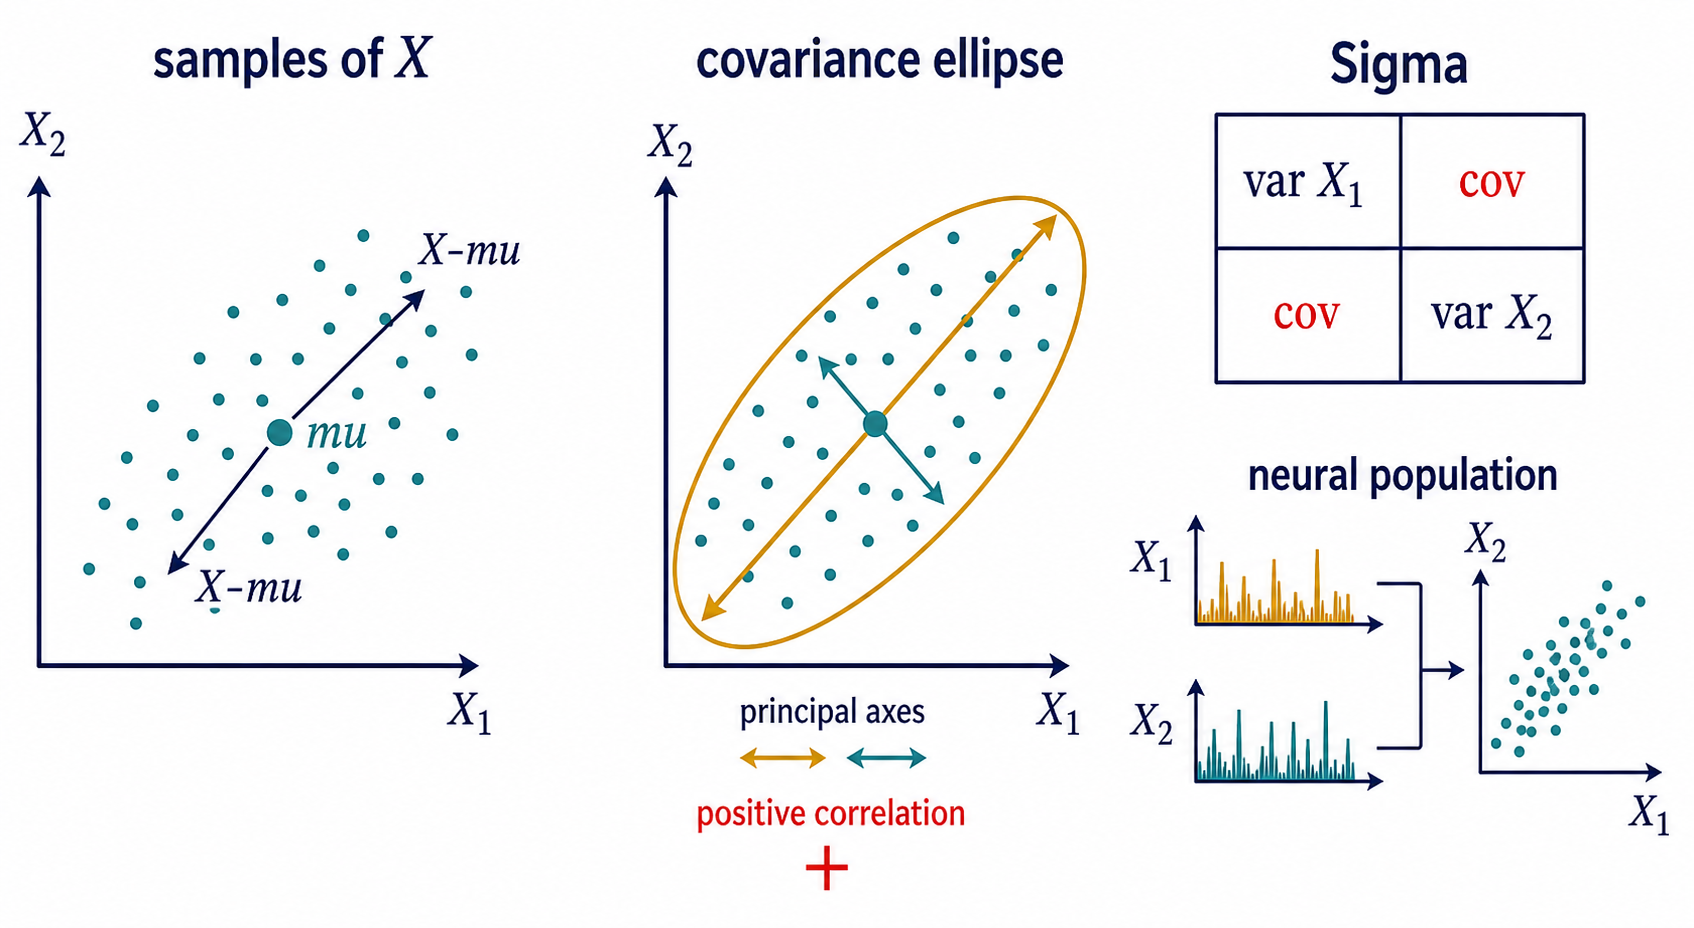
\includegraphics[width=0.98\linewidth]{imagegen-figures/ch13-random-vectors-covariance.png}
\caption{A random vector produces vector-valued samples. The mean \(\mu\) marks the center, deviations \(X-\mu\) point from the center to samples, and the covariance matrix \(\Sigma\) summarizes spread and co-movement. In two dimensions, covariance appears as an ellipse whose principal axes point along high- and low-variance directions.}
\label{fig:ch13-random-vectors-covariance}
\end{figure}

\paragraph{Formal setup.}
Let \(X:\Omega\to\mathbb{R}^d\) be a random vector with components \(X_1,\ldots,X_d\). Assume the needed expectations exist. The mean vector is
\[
\mu=\mathbb{E}[X]
=
\begin{bmatrix}
\mathbb{E}[X_1]\\
\vdots\\
\mathbb{E}[X_d]
\end{bmatrix}.
\]
The covariance matrix is
\[
\boxed{\Sigma=\operatorname{Cov}(X)=\mathbb{E}\!\left[(X-\mu)(X-\mu)^\top\right].}
\]
Its entries are
\[
\Sigma_{ij}
=
\operatorname{Cov}(X_i,X_j)
=
\mathbb{E}\!\left[(X_i-\mu_i)(X_j-\mu_j)\right].
\]
The diagonal entries are variances:
\[
\Sigma_{ii}=\operatorname{Var}(X_i).
\]
When variances are positive, the correlation between coordinates \(i\) and \(j\) is
\[
\rho_{ij}
=
\frac{\Sigma_{ij}}{\sqrt{\Sigma_{ii}\Sigma_{jj}}}.
\]
For data samples \(x_1,\ldots,x_n\in\mathbb{R}^d\), the sample mean and sample covariance are
\[
\widehat{\mu}=\frac1n\sum_{k=1}^n x_k,
\qquad
\widehat{\Sigma}=\frac1{n-1}\sum_{k=1}^n (x_k-\widehat{\mu})(x_k-\widehat{\mu})^\top.
\]

\paragraph{Core intuition.}
Figure~\ref{fig:ch13-random-vectors-covariance} links random vectors to geometry from Chapters 3-6. Each observed vector is a point. The mean is the center. A deviation \(X-\mu\) is an arrow from the center to a sample. The covariance matrix averages outer products of those deviation arrows.

In two dimensions, a cloud with positive covariance tilts upward: when \(X_1\) is above its mean, \(X_2\) tends to be above its mean too. A negative covariance tilts downward. A covariance near zero means no linear co-movement, but nonlinear dependence may remain. The covariance ellipse shows directions of high and low variance; its axes are related to eigenvectors of \(\Sigma\), which connects directly to PCA from Chapter 6.

Beginners often confuse covariance with causation. Covariance says coordinates vary together under a distribution. It does not say one coordinate causes the other. Covariance also depends on units: changing milliseconds to seconds rescales variances and covariances. Correlation removes units by normalizing, but it still measures only linear association.

This section previews expectation, which Chapter 15 will define more fully as an averaging operator. It prepares Chapter 14's multivariate Gaussian, Chapter 16's high-dimensional probability, Chapter 17's uncertainty estimates, and Chapter 18's Fisher information geometry.

\paragraph{Main theorem: covariance matrices are symmetric positive semidefinite.}
If \(X\in\mathbb{R}^d\) has covariance matrix \(\Sigma\), then
\[
\Sigma^\top=\Sigma
\]
and, for every vector \(a\in\mathbb{R}^d\),
\[
a^\top\Sigma a\geq0.
\]

\emph{Proof sketch.}
Symmetry follows from the entries:
\[
\Sigma_{ij}
=\mathbb{E}[(X_i-\mu_i)(X_j-\mu_j)]
=\mathbb{E}[(X_j-\mu_j)(X_i-\mu_i)]
=\Sigma_{ji}.
\]
For positive semidefiniteness, use the central covariance equation:
\[
a^\top\Sigma a
=
a^\top\mathbb{E}[(X-\mu)(X-\mu)^\top]a.
\]
Linearity of expectation allows the fixed vector \(a\) to move inside:
\[
a^\top\Sigma a
=
\mathbb{E}\!\left[a^\top(X-\mu)(X-\mu)^\top a\right].
\]
The scalar inside is
\[
a^\top(X-\mu)(X-\mu)^\top a
=
\left(a^\top(X-\mu)\right)^2.
\]
Therefore
\[
a^\top\Sigma a
=
\mathbb{E}\!\left[\left(a^\top X-a^\top\mu\right)^2\right]
=
\operatorname{Var}(a^\top X)\geq0.
\]
The mechanism is geometric: covariance cannot assign negative variance to any one-dimensional projection.

\paragraph{Worked examples.}
\emph{Small numerical example.} Let \(Z=(X,Y)^\top\), where \(X,Y\in\{0,1\}\), with joint table
\[
\begin{array}{c|cc}
&Y=1&Y=0\\
\hline
X=1&0.40&0.10\\
X=0&0.20&0.30
\end{array}
\]
from Section 13.3. Then
\[
\mathbb{E}[X]=0.50,
\qquad
\mathbb{E}[Y]=0.60,
\qquad
\mathbb{E}[XY]=0.40.
\]
Thus
\[
\operatorname{Var}(X)=0.50(1-0.50)=0.25,
\]
\[
\operatorname{Var}(Y)=0.60(1-0.60)=0.24,
\]
and
\[
\operatorname{Cov}(X,Y)=\mathbb{E}[XY]-\mathbb{E}[X]\mathbb{E}[Y]
=0.40-(0.50)(0.60)=0.10.
\]
The covariance matrix is
\[
\Sigma=
\begin{bmatrix}
0.25&0.10\\
0.10&0.24
\end{bmatrix}.
\]
The positive off-diagonal entries say that \(X\) and \(Y\) tend to be large together more often than independence would predict.

\emph{ML/neuroscience example.} Suppose \(X\in\mathbb{R}^{100}\) is a vector of spike counts from \(100\) neurons in one time bin. The mean vector \(\mu\) stores the average firing rate of each neuron. The entry \(\Sigma_{ij}\) stores the trial-to-trial co-variability of neurons \(i\) and \(j\). A large positive \(\Sigma_{ij}\) means the two neurons tend to fluctuate above and below their means together. PCA applied to \(\Sigma\) finds directions in population activity with large variance, which can reveal low-dimensional neural state structure.

\paragraph{ML/DL/neuroscience connections.}
In machine learning, covariance matrices summarize feature spread, whitening transformations, PCA, Gaussian approximations, optimizer preconditioners, and uncertainty estimates. In deep learning, activation covariance describes how representation coordinates co-vary across examples; batch normalization and whitening-like methods use related second-order summaries. In neuroscience, the covariance matrix becomes neural population covariance: coordinates are neurons, samples are trials or time bins, diagonal entries are single-neuron variability, and off-diagonal entries are noise correlations or shared state fluctuations.

\paragraph{Exercises.}
\begin{enumerate}[label=\textbf{13.4.\arabic*.}, leftmargin=*]
\item \textbf{Mechanical.} A random vector \(X=(X_1,X_2)^\top\) has \(\mathbb{E}[X_1]=1\), \(\mathbb{E}[X_2]=2\), \(\mathbb{E}[X_1^2]=5\), \(\mathbb{E}[X_2^2]=8\), and \(\mathbb{E}[X_1X_2]=4\). Compute \(\operatorname{Var}(X_1)\), \(\operatorname{Var}(X_2)\), \(\operatorname{Cov}(X_1,X_2)\), and \(\Sigma\).
\item \textbf{Proof or derivation.} Prove that \(\operatorname{Cov}(X_i,X_j)=\mathbb{E}[X_iX_j]-\mathbb{E}[X_i]\mathbb{E}[X_j]\), assuming the relevant expectations exist.
\item \textbf{Numerical/computational.} For samples \(x_1=(1,2)^\top\), \(x_2=(2,1)^\top\), \(x_3=(3,4)^\top\), and \(x_4=(4,3)^\top\), compute the sample mean and sample covariance using the \(1/(n-1)\) formula.
\item \textbf{Interpretation.} A two-neuron covariance ellipse is long along the direction \((1,1)\) and short along \((1,-1)\). What does this say about shared fluctuations in the two neurons?
\item \textbf{Debug the misconception.} A student says, "If covariance is zero, the variables must be independent." Give a counterexample idea, such as a symmetric variable \(X\) and \(Y=X^2\), and explain what covariance fails to detect.
\end{enumerate}

\paragraph{Closing bridge.}
This chapter made uncertainty precise by turning events into measurable sets, random variables into functions, distributions into pushforward measures, and covariance into matrix geometry. Chapter 14 builds a structured catalog of probability laws. Chapter 15 then returns to expectation and conditioning as the main operations for prediction, inference, and decision-making under uncertainty.

\clearpage
